\section{Metodi con reti neurali}

    \begin{frame}{Autoencoder}
        \begin{figure}[t!]
            \centering
            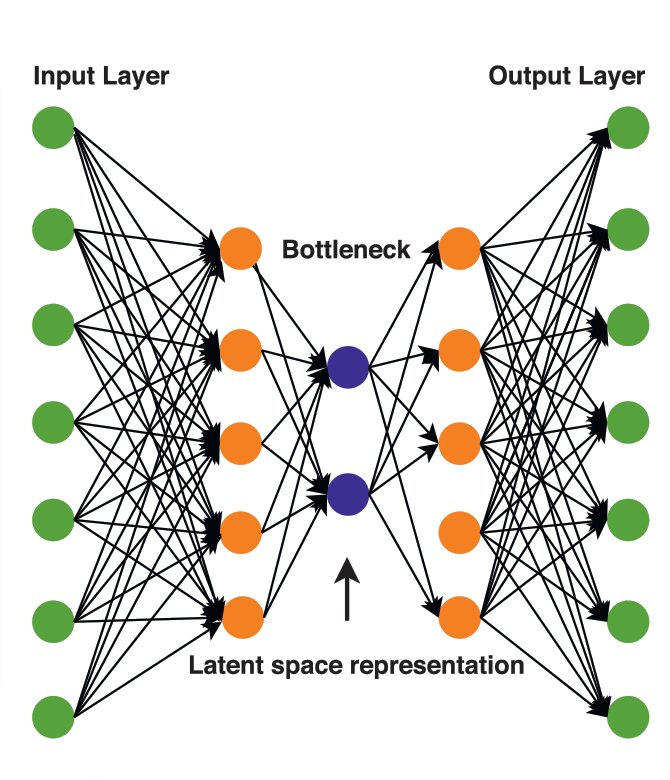
\includegraphics[width=0.5\textheight]{Immagini/Autoencoder_scheme.png}
            \caption{Schema generico di un autoencoder, immagine presa dal documento \textit{Deep architectures for image compression: A critical review}\footnotemark[1]}
            \label{fig:schemeAutoencoder}
        \end{figure}
        \footnotetext[1]{\fullcite{mishra2022deep}}
    \end{frame}

    \begin{frame}{Metodi con reti neurali}
        I metodi di codifica con reti neurali analizzati in questo studio sono i seguenti
        \begin{itemize}
            \item Variational compression with a scale hyperprior, Ballé et al\footnotemark[1].
            \item Discretized gaussian mixture likelihoods, Cheng et al\footnotemark[2].
            \item Neural data-dependent transform, Wang et al\footnotemark[3]. 
        \end{itemize}
        \footnotetext[1]{\fullcite{minnen2018joint}}
        \footnotetext[2]{\fullcite{cheng2020learned}}
        \footnotetext[3]{\fullcite{wang2022neural}}
    \end{frame}

    \begin{frame}{Ballé et al\footnotemark[1]. 2018}
        \begin{figure}[!h]
            \centering
            \includegraphics[width=0.7\textheight]{Immagini/Ballé2018_Rete.png}
            \caption{Diagramma rete Ballé 2018 et al., immagine presa dal documento \textit{Joint autoregressive and hierarchical priors for learned image compression}\footnotemark[1]}
            \label{fig:balle2018Network}
        \end{figure}
        \footnotetext[1]{\fullcite{minnen2018joint}}
    \end{frame}

    \begin{frame}{Cheng et al\footnotemark[1]. 2020}
        \begin{figure}[!h]
            \centering
            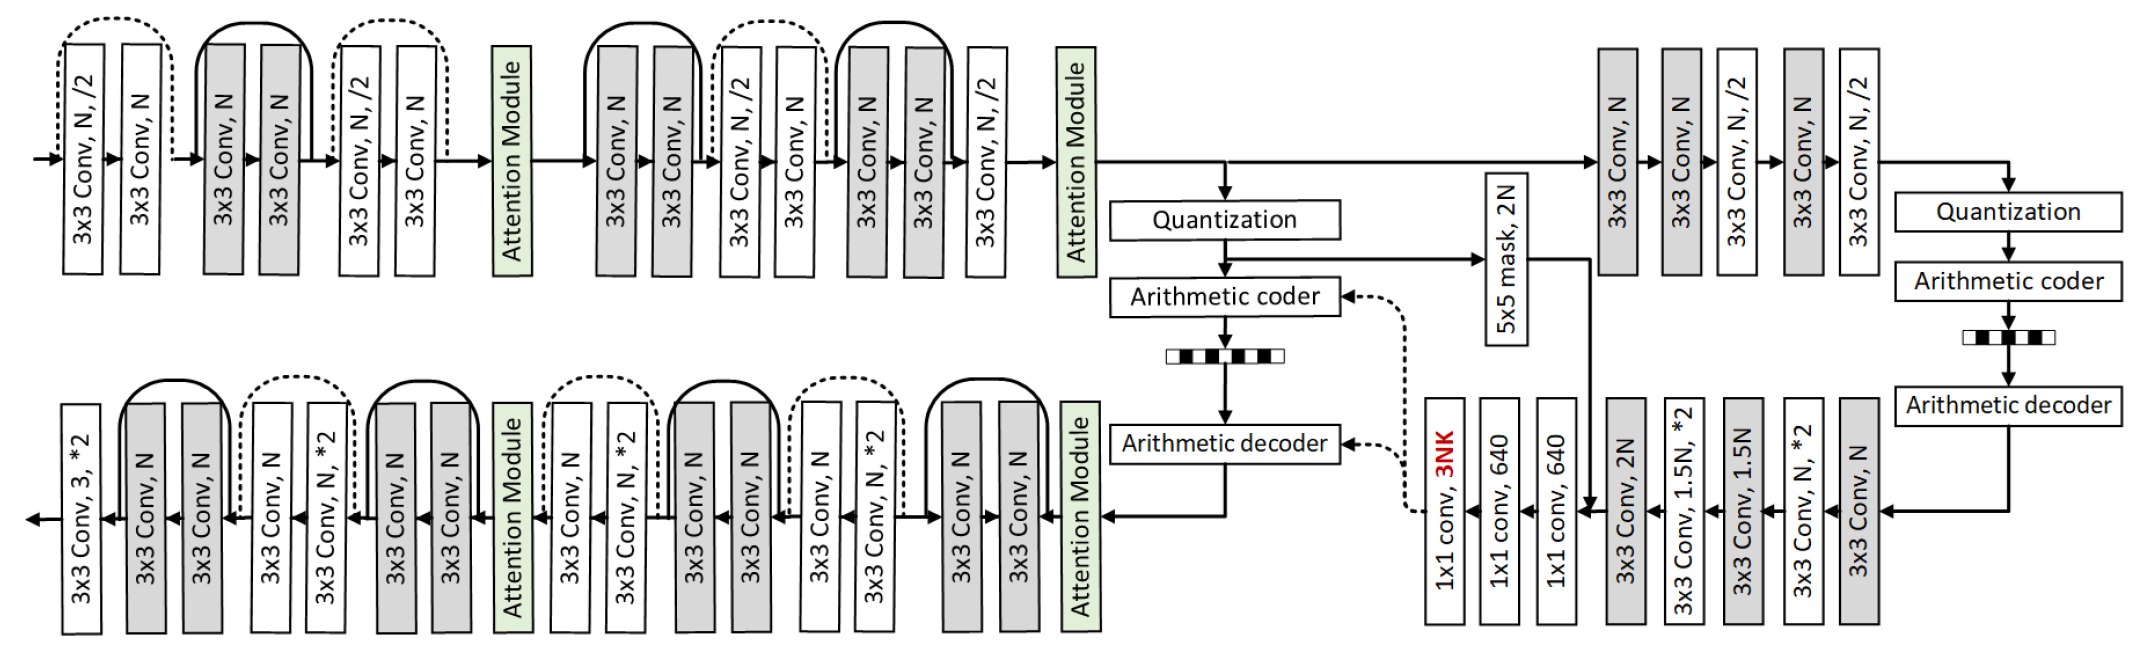
\includegraphics[width=1\textwidth]{Immagini/Cheng2020_Rete.png}
            \caption{Diagramma rete Cheng 2020 et al., immagine presa dal documento \textit{Learned image compression with discretized gaussian mixture likelihoods and attention modules}\footnotemark[1]}
            \label{fig:cheng2020Network}
        \end{figure}
        \footnotetext[1]{\fullcite{cheng2020learned}}
    \end{frame}

    \begin{frame}{Wang et al\footnotemark[1]. 2022}
        \begin{figure}[!h]
            \centering
            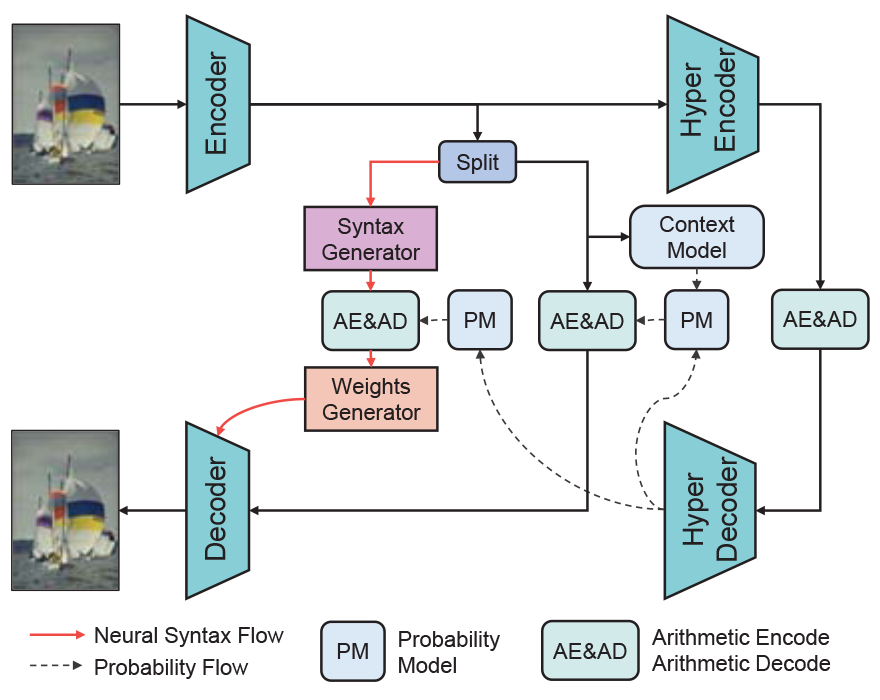
\includegraphics[width=0.6\textheight]{Immagini/Wang2022_Rete.png}
            \caption{Diagramma rete Wang 2022 et al., immagine presa dal documento \textit{Neural data-dependent transform for learned image compression}\footnotemark[1]}
            \label{fig:Wang2022Network}
        \end{figure}
        \footnotetext[1]{\fullcite{wang2022neural}}
    \end{frame}
    